\noindent A characteristic feature of eukaryotic cells is the presence of multiple internal membrane-bounded compartments. 
%
These compartments exchange molecules amongst themselves in small membrane-bounded packets called vesicles ~\cite{alberts2002molecular}. 
%
The molecular interaction network that controls the vesicle transport system involves dozens of varieties of molecules that regulate flow of cargo. 
%
Due to this, obtaining a complete understanding of the vesicle transport system through physical experimentation alone is a hard problem.
%
Highly reduced models of vesicle traffic have previously provided insight into how the chemical composition of various cellular compartments can emerge out of molecular regulation and cargo flow. 
%
However, high complexity of problems in VTS also restricts the use of traditional methods like simulation and statistical reasoning~\cite{mani2016wine, mani2016stacking}. 
%The high complexity of problem restricts the use of traditional methods like simulation and statistical reasoning and the requirement of precise analysis makes formal methods an ideal candidate. 
In this paper, using formal methods, we solve the problem of completing incomplete VTS graphs while also considering constraints due to molecular interactions, thereby demonstrating the effectiveness of such methods.

The phenomenology of vesicle traffic is unlikely to be familiar to many readers; however, the details are important for the rest of our discussion. 
%
Therefore, we give an overview of the molecular mechanism of the VTS and then we sketch out a few interesting problems that are key to an understanding of the VTS.

\subsection{Vesicle traffic system}
%Vesicles were discovered decades ago, in the early 1950s, and s
\noindent The major molecules involved in the vesicle traffic system~\cite{wells2005discovery} can roughly be categorized as budding molecules, whose role is in the formation and budding of transport vesicles from the source compartment, and fusion molecules, which enable fusion of transport vesicles with the target compartments. 
%
Below, we give a brief description of the sequence of steps involved in the vesicle transport process. 
%
Through this description, we wish to provide a glimpse of the kind of molecular regulatory interactions that we encode in our model.
 
\begin{figure}
	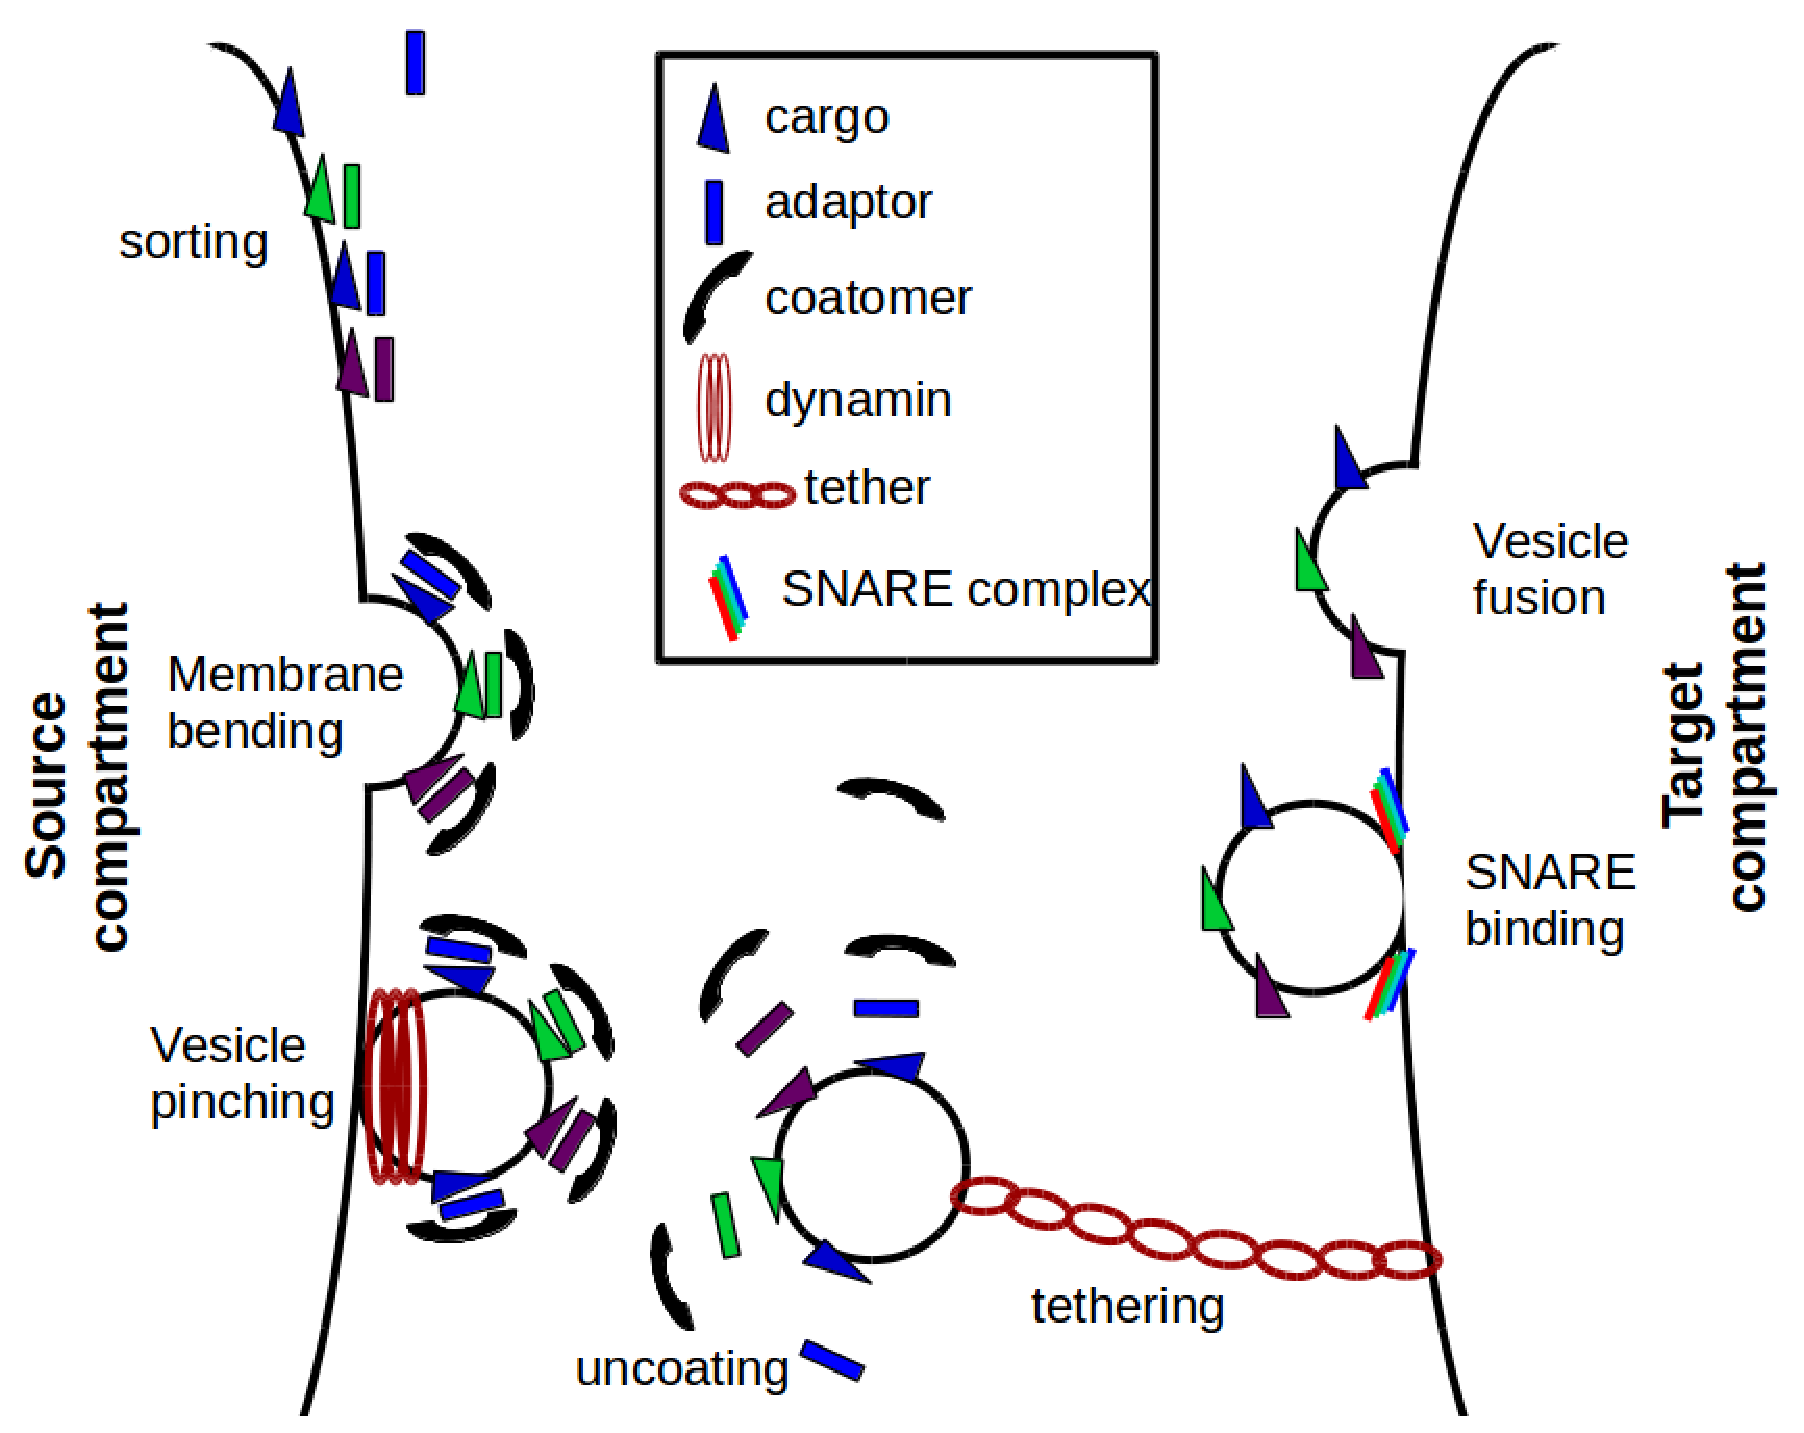
\includegraphics[height=10cm,width=12cm]{diavts.eps}
	\caption{Schematic of the vesicle transport system. Steps involved in vesicle transport between two compartments: a source and a target compartment are shown. 
	%
	The symbols used for different molecules involved in vesicle traffic are explained in the key. At the source compartment, transmembrane cargo proteins are sorted by cytosolic adaptor proteins. 
	%
	Here, the different colours indicate different types of cargo and adaptor proteins. Coat proteins are recruited to the forming vesicle by adaptor proteins. 
	%
	Note here that a single type of coat protein can interact with multiple types of adaptor proteins. Subsequently, the vesicle is pinched off at its neck, for example by dynamin. 
	%
	Once the vesicle has left the source compartment, the coat and adaptor proteins fall off and the vesicle is recognized and bound by a tethering complex which is linked to the target compartment. 
	%
	At the target compartment the tethered vesicle undergoes fusion, thereby releasing its contents.}
    \label{fig:vts}
\end{figure}

\subsubsection{Vesicle budding} The process of vesicle budding involves sorting and packaging of cargo molecules, membrane deformation and budding of the vesicle from the source compartment~\ref{fig:vts}.
%
Cargo sorting is performed by cytosolic adaptor proteins. 
Adaptors are recruited to the source compartment through interactions with the lipids that form the compartment's membrane, and interactions with molecular switches called Arf/Sar which signal the initiation of vesicle formation~\cite{paczkowski2015cargo}. 
%
Then these adaptors bind to cargo molecules and thereby sequester them for packaging. 
%
Different adaptor proteins act at different compartments, for example, vesicle formation at the ER requires the adaptor sec23/24, and the AP2 adaptor is used for packaging vesicles at the plasma membrane.
%

The next step is membrane deformation, which involves cytosolic coat proteins. 
%
Coat proteins are recruited to the forming vesicle through their interaction with adaptor proteins. 
%
These are naturally curved proteins, and their assembly on membranes leads to membrane deformation.
%
A single kind of coat protein can bind to multiple kinds of adaptors, thereby allowing the packaging of multiple types of cargo within the same vesicle. 
%
There are three major types of coat proteins: Clathrin, COP2 and COP1. These act on different compartments: the clathrin coat operates at multiple compartments, and can interact with multiple adaptors proteins, whereas the COP2 and COP1 coat are only involved in vesicle formation at a single compartment: the ER and the Golgi respectively~\cite{faini2013vesicle}.
%
Finally, transport vesicles bud out from the source compartment~\cite{cocucci2014dynamin}.
%
The vesicle is now ready for transport and subsequent fusion with a target compartment.

\subsubsection{Vesicle fusion} The vesicle fusion involves two steps recognition of the correct target compartment and fusion of the transport vesicle~\ref{fig:vts}.

Target compartment recognition involves molecular switches called Rabs and  tethering complexes. Distinct compartments of the cell are associated with distinct Rabs. For example, Rab5 is associated early endosomes and  Rab7 with late endosomes\cite{rink2005rab}.  
%
Rabs are master regulators; in their active form Rabs recruit many downstream proteins, including tethering complexes, fusion regulators, motor proteins, etc, to their compartment ~\cite{muller2018molecular}.

Tethering complexes sequester vesicles to their target compartments by binding to the vesicle on one end and the target compartment on the other end, thereby bridging the two before fusion. 
%
They are also believed to function as chaperones for assembly of SNARE protein complexes, which enable vesicle fusion. 
%
A clear mechanism for action of these tethers is missing, but evidence from experiments indicate that tethers bind to vesicles through molecular interactions with vesicle coat proteins, vesicle, associated Rabs, SNAREs and SNARE regulators. 
%
They can also sense membrane curvature (vesicles are highly curved) ~\cite{baker2016chaperoning}.

The final step in vesicle transport is fusion of vesicle with the target compartment is brought about by SNARE proteins. 
%
There are four kinds of SNAREs: R, Qa, Qb, and Qc; and vesicle fusion requires formation of a SNARE complex containing one of each type. 
%
In all known cases, one SNARE protein of the complex is contributed by the vesicle and the other three SNAREs by the target compartment. 
%
A few SNARE proteins, such as SNAP25, contain both Qb- and Qc-SNARE motifs~\cite{yoon2018snare}.

%\somya{schematic of snare regulatory network}
\subsubsection{Schematic of snare regulatory network}
In keeping with their central role in vesicle transport, both the activity and the localization of SNARE proteins are regulated. Notable regulators are Sec17/18 and the SM proteins.
%
Sec17/18 bring about disassembly of SNARE complexes post-fusion in order that these SNAREs may be reused. 
%
Whereas, SM proteins have following multiple modes of SNARE regulation: 
\begin{itemize}
	\item SM proteins can hold
	the Qa-SNAREs in an inhibited state and prevent or postpone their assembly into SNARE
	complexes.
	%
	\item Some SM proteins can act as a template upon which an early SNARE complex intermediate can
	form.
	%
	\item Finally, SM proteins bind the fully assembled
	SNARE complexes to protect them from premature disassembly by Sec17/18~\cite{baker2016chaperoning}.
	%
	\item SM proteins have also been shown to interact with tethers~\cite{yoon2018snare}.
\end{itemize}

%\somya{schematic of intracellular compartments and  major routes}
\subsubsection{Major paths in the vesicle transport network}
Molecules traverse the cell in a series of vesicles, and there are two major routes of vesicle transport in all eukaryotic cells.
%
\begin{itemize}
	\item The secretory route takes proteins from the ER (their site of production) to the plasma membrane( from where they are secreted out of the cell) via the Golgi apparatus\cite{alberts2002molecular}.
	%
	\item The endocytic route takes proteins from the outside of the cell, through the plasma membrane, to the endocytic compartments and the lysosome where they are digested. 
\end{itemize}
Other paths are used for cross talk between the secretory and the endocytic routes. For example, vesicles are sent back and forth between the Trans-Golgi network (secretory route) to the early and the late endosomes(endocytic route)\cite{progida2016bidirectional}. Also, recently, unconventional vesicle-mediated secretory routes have been found, which bypass the Golgi apparatus. The molecules involved in these routes are as yet unknown\cite{nickel2018unconventional}. 
%
%\begin{table}
%	\begin{center}
%		\begin{tabular}{|c|c|c|c|c|c|c|c|c|c|c|}
%			\hline
%			Nodes & 1 & 2 & 3 & 4 & 5 & 6 & 7 & 8 & 9 & 10 \\ \hline
%			Graphs & 0 & 0 & 0 & 1 & 2 & 15 & 121 & 2159 & 68715 & 3952378 \\ 
%			\hline
%		\end{tabular}
%		\label{tab:threec}
%		\caption{Number of simple 3-edge-connected unlabelled N-node graphs.}
%	\end{center}	
%\end{table}

\subsection{The model}
\noindent The VTS model for this paper is inspired by~\cite{shukla2017discovering}. 
%
On the timescales of minutes, we have tried to capture important aspect of Rothman-Schekman-Sudhof (RSS) model~\cite{rothman2002machinery} of vesicle traffic system.
%
The following are the basic component and assumptions of our model. 
\begin{enumerate}
\item A cell is a set of compartments exchanging vesicles.
\item Compartments are neither created nor destroyed~\cite{braell1984glycoprotein}.
\item Each compartment is in steady state, gain and loss of the molecules is balance~\cite{braell1984glycoprotein}.
\item Molecules are neither created nor destroyed~\cite{he2009differential}.
\item Molecules move via vesicles of uniform size.
\item Identical vesicles have identical target compartments~\cite{fries1981transient}.
\item Fusion of vesicles to compartments is driven by specific SNARE pairing~\cite{mcnew2000compartmental}.
%\item The identities of compartments and vesicles is encoded in their molecules, and identical vesicles fuse with identical target compartments.
\item The activity of a SNARE can be regulated by other molecules present on the same compartment or vesicle~\cite{mima2008reconstituted}.
\item An active SNARE pair is necessary and sufficient for fusion~\cite{weber1998snarepins}
. 
\end{enumerate}
%
All our assumptions, except assumption 5, are held up by cell biological results.
%
Although vesicles produced in a cell do vary in size~\cite{jena2008intracellular}, they are much smaller than compartments, hence, for the sake of simplicity, we assume a uniform size for intracellular vesicles.
%The assumptions 
%On the timescale of minutes, compartments are neither created nor destroyed, rather, they are in steady state. We assume that molecules are also neither created nor destroyed.
%The activity of a SNARE can be regulated by other molecules present on the same compartment or vesicle.

\subsection{Abstraction of VTS as a graph problem}

%In this section, we will describe the basic constraints imposed by cell biology. These are all incorporated into an abstract model of a VTS, whose properties will then be explored using SMT solvers.

\noindent In this section, we will abstract from the biological description of the VTS and represent the whole network as an annotated transport graph. 
%
The constraints imposed by cell biology are incorporated in the  annotations of the graph. 

\subsubsection{The cell as a transport graph} 
%We consider a cell to be a collection of compartments (nodes) and vesicles (edges), thus defining a transport graph. Every compartment or vesicle has a set of molecular labels, such as SNARE proteins, associated with it.
The cell can be abstractly represented as an annotated graph. 
Every compartment in the cell can be represented as a node in the graph. 
%
The set of molecules present in the compartment, for example, SNARE proteins associated with it, are represented as a label to the corresponding nodes.
%
The label of each node will be unique molecules present on the compartment, i.e we abstract over the quantity of the molecule present in a compartment.
%This represents the flux of the molecule type present at that compartment.
%
The transport vesicle flowing from source compartment to the target compartment is represented by a labeled directed edge. 
% 
The label represents the associated flux of all molecular types carried by the corresponding vesicle.
%
%

\subsubsection{Steady state} 
The vesicle transfer will change the molecular composition (distinct molecule count) on both the source compartment and the target compartment. 
%
In our model, we assume that the cell is in steady state. As a further simplification, we also assume that the incoming and outgoing flux is balanced for each of the molecular types at each compartment. 
Indeed, it is well accepted that on the scale of minutes and hours the molecular composition remains the same. 
%
In this paper, we refer to the steady state of the cell (referred to as \textit{homeostasis} in biological literature) as the stability condition over the annotated graph.


%Each edge is associated with a flux of all the molecular types carried by the corresponding vesicle. The total amount of each molecular type on each compartment can therefore increase or decrease. We assume the cell is in a steady state where each compartment’s composition does not vary over short time scales. Therefore, incoming and outgoing fluxes are balanced for each molecular type at each compartment; it is the \textit{stability cond1ition}.

\subsubsection{Vesicle fusion}
%Based on the earlier discussion of fusion, the vesicle targeting is driven by molecular interactions.  
%
%Particularly, molecules composition (SNARE proteins etc) present on the budded vesicle determines it's properties, which 
% 
%The molecular composition and hence the properties of the transfer vesicle 
%is the crucial factor to which target compartment the vesicle will fuse to.
%
%For any given pair of a vesicle and a compartment, the SNARE proteins present on both influence the fusion of the vesicle to that compartment.
%  
%Biophysically, fusion of a vesicle to the target compartment requires a direct physical interaction between at least one SNARE type on the vesicle and one SNARE type on the compartment.
%
%Once a vesicle has budded out of the source, the molecules it carries determine its properties. In particular, for any given pair of a vesicle and a compartment, the set of SNARE proteins that label the former and latter influence whether the vesicle will fuse to that compartment. Biophysically, fusion requires a direct physical interaction between at least one SNARE type on the vesicle and one SNARE type on the compartment. 
%
%SNAREs are of two types (known as Q and R in the cell biology iterature) and 
Vesicle fusion requires a pairing of 3 Qsnares and 1 Rsnare that are distributed between the transfer vesicle and the target compartment. 
%For any given pair of a vesicle and a compartment, vesicle fusion requires a pairing of a Q-SNARE with an R-SNARE on 
%the SNARE proteins present on both influence the fusion of the vesicle to that compartment.
%
%The list of molecular pairs that can drive a fusion event is given in a pairing matrix between Q and R SNAREs. 
%
Not all sets of Q and R SNAREs are allowed to fuse with each other.
%
In the model, we assume that the cell has an equal number of Q and R SNARE types.
%
Therefore, we can abstract the underlying cell biology by labeling the nodes and edges with an equal number of Q and R SNAREs. 
% equal number of Q and R SNAREs as a part of node and edge label.
%
%
Given a relation of all allowed fusion SNARE pairings, we can computationally determine whether a particular transfer vesicle will fuse to a particular target compartment (the edge between two compartments) based on the above condition.  

\subsubsection{Molecular regulation} 
Fusion takes place only if the SNARE types involved in the vesicle and compartment are both in an active state.
%We assume that for fusion to occur, the pair of 
%
The activity of these SNAREs is dependent on the presence of other molecules on the vesicle or compartment, respectively.
%
In our abstract model, 
we create a hierarchy of models for varying degrees of regulation of SNARE activity.
%we create a set of variations of different kind of molecular regulations.
%
Most generally, the activity state of a given SNARE can be a Boolean function of all the molecular types on a compartment or vesicle. 
%
We have also tested \cite{shukla} a particularly simple regulation mechanism in which two SNAREs that can pair to drive fusion to inhibit one another; this is the \textit{pairing inhibition}. 
%
This is motivated by the idea that pairing must generate an inactive bi-molecular complex.
%

%We assume that for fusion to occur, the pair of SNARE types involved on the vesicle and compartment must both be in an active state. Whether these SNAREs are active or inactive depends on the other molecules found on the vesicle or compartment, respectively. We test many different versions of this kind of molecular regulation. Most generally, the activity state of a given SNARE can be a Boolean function of all the molecular types on a compartment or vesicle. We have also tested \cite{shukla} a particularly simple regulation mechanism in which two SNAREs that can pair to drive fusion inhibit one another; this is the \textit{pairing inhibition}. This is motivated by the idea that pairing must generate an inactive bi-molecular complex.

%\textbf{Difficulty of the analysis:}

%
%Properties of the VTS would be hindered by the same reason. 
%3-connected graphs and all possible variations of SNARE regulation rules. 
%
%The number of graphs of specified connectivity grows exponentially with the number of nodes: Table~\ref{tab:threec} shows how many 3-edge-connected graphs~\cite{a052448-oeis} exist (without parallel or self edges) as node number N increases.
\subsection{Graph connectivity is an interesting and accessible property of the VTS} 
%\textbf{Properties of a VTS that satisfies all cell-biological constraints:} 
\noindent Interactions between the molecules of the VTS together produce a functional vesicle transport network, in which molecules flow between intracellular compartments using specified paths.
%
The molecules of the VTS, their interactions and modes of regulation have been worked out to a large extent through cell-biological experiments. 
%
But we do not know if this information is complete. In order to assess how completely we know the VTS, we need easily readable benchmarks. 

%\ankit{Need more clarity on the importance and relevance of the CONNECTIVITY and it's relevance.}
One such benchmark is provided by our result about connectivity of the VTS graph. Graph connectivity is defined as the minimum number of edges that need to be removed from an undirected graph to render it disconnected. For example, in a directed cyclic graph, every node has at least one incoming and one outgoing edge, at least 2 edges need to be removed in order to disconnect the graph. Therefore the underlying undirected graph is 2-connected. 
From our result, for a given set of biomolecular interactions, for a cell that is in steady state, we expect the VTS graph to have a certain k-connectivity. When regulation is given by arbitrary Boolean rules,   we find that VTS graphs must be 3-connected. And when we add the constraint of the specific form of regulatory interactions seen between VTS molecules, we expect vesicle transport graphs to be 2-strongly connected [28].

%\ankit{We need not specify Synthesis here. Only connectivity use next subsection to build this.}
%\somya{But this is the para where we explain why connectivity is interesting an biological property}
%\ankit{Yes; Both of our remark looks correct!}
The vesicle transport graphs available today for eukaryotic organisms are incomplete themselves. 
%
In this situation, we use our result as a tool to predict missing edges which satisfy the graph connectivity constraint. 
%
These predictions are intended to be used as guides for future experiments. 
%
A mismatch between our predictions and experiments would indicate that our current understanding of the VTS molecules is necessarily incomplete. 
%
Note that, on the other hand, if our predictions are experimentally confirmed, it does not imply that our understanding of the VTS is complete.\\
%

\begin{example}
%
In figure~\ref{fig:M1}, we present a VTS that has 3 compartments and 8 molecules, and a corresponding pairing matrix.
%
Molecules are numbered 0-7.
%
In the VTS, labels are a string of molecule ids, and an overline over an id indicates that the molecule is active.
%
Every molecule on the node is active.
%
The activity of the molecules on an edge are controlled
by presence of the other molecules on the edge.
%
On the right side of the figure, we show the pairing matrix.
%
An entry 1 represents pairing between molecules.
%
$\times$ represents no pairing.
%
Rows corresponds to the labels of edges, and
columns corresponds to the labels of nodes.
%
Every molecule flows on a cycle, ensuring steady state.
%
This is a 3-connected graph.
\end{example}
%
\begin{figure}
\centering
\begin{minipage}{0.50\linewidth}
  \hspace{-4ex}
\begin{tikzpicture}
\matrix [matrix of math nodes,left delimiter=(,right delimiter=),row sep=0.16cm,column sep=0.1cm] (m) {
\times & \times & \times &\times&\times&\times & \times & \times\\
\times & \times & \times&\times&\times&\times& 1 &\times \\
\times & \times & \times&\times&\times&1&\times &\times\\
\times & \times & \times&\times & 1 & \times &\times & \times\\
 \times & \times & \times & \times & \times & \times & \times & \times\\
 \times & \times & \times &\times & \times & \times & \times & \times\\
 \times & \times & \times & \times & \times & \times & \times & \times\\
 \times & \times & \times & \times & \times & \times&\times & \times\\};

\draw[dashed] ($0.5*(m-1-4.north east)+0.5*(m-1-5.north west)$) --
     ($0.5*(m-8-5.south east)+0.5*(m-8-4.south west)$);

\draw[dashed] ($0.5*(m-4-1.south west)+0.5*(m-5-1.north west)$) --
 ($0.5*(m-4-8.south east)+0.5*(m-5-8.north east)$);

\node[above=4pt of m-1-1] (top-1) {$M_1$};
\node[above=4pt of m-1-2] (top-2) {$M_2$};
\node[above=4pt of m-1-3] (top-3) {$M_3$};
\node[above=4pt of m-1-4] (top-4) {$M_4$};
\node[above=4pt of m-1-5] (top-5) {$M_5$};
\node[above=4pt of m-1-6] (top-6) {$M_6$};
\node[above=4pt of m-1-7] (top-7) {$M_7$};
\node[above=4pt of m-1-8] (top-8) {$M_8$};

\node[left=12pt of m-1-1] (left-1) {$M_1$};
\node[left=12pt of m-2-1] (left-2) {$M_2$};
\node[left=12pt of m-3-1] (left-3) {$M_3$};
\node[left=12pt of m-4-1] (left-4) {$M_4$};
\node[left=12pt of m-5-1] (left-5) {$M_5$};
\node[left=12pt of m-6-1] (left-6) {$M_6$};
\node[left=12pt of m-7-1] (left-7) {$M_7$};
\node[left=12pt of m-8-1] (left-8) {$M_8$};


\node[rectangle,above delimiter=\{] (del-top-1) at ($0.5*(top-1.south) +0.5*(top-4.south)$) {\tikz{\path (top-1.south west) rectangle (top-4.north east);}};
\node[above=10pt] at (del-top-1.north) {$Q-Snares$};
\node[rectangle,above delimiter=\{] (del-top-2) at ($0.5*(top-5.south) +0.5*(top-8.south)$) {\tikz{\path (top-4.south west) rectangle (top-6.north east);}};
\node[above=10pt] at (del-top-2.north) {$R-Snares$};

\node[rectangle,left delimiter=\{] (del-left-1) at ($0.5*(left-1.east) +0.5*(left-4.east)$) {\tikz{\path (left-1.north east) rectangle (left-4.south west);}};
\node[left=15pt,rotate=90,xshift=9mm] at (del-left-1.west) {$Q-Snares$};
\node[rectangle,left delimiter=\{] (del-left-2) at ($0.5*(left-5.east) +0.5*(left-8.east)$) {\tikz{\path (left-5.north east) rectangle (left-8.south west);}};
\node[left=15pt,rotate=90,xshift=9mm] at (del-left-2.west) {$R-Snares$};

\begin{pgfonlayer}{myback}

\foreach \element in {m-1-7,m-3-8,m-5-1,m-5-2,m-5-3,m-5-4,m-6-1,m-6-2,m-6-3,m-6-4,m-7-1,m-7-2,m-7-3,m-7-4,m-8-1,m-8-2,m-8-3,m-8-4}{
\highlight[pink]{\element}{\element}
}
\foreach \element in {m-2-7,m-3-6,m-4-5}{
\fhighlight[blue!10]{\element}{\element}
}
\end{pgfonlayer}

\end{tikzpicture}  
\end{minipage}
\begin{minipage}{0.45\linewidth}

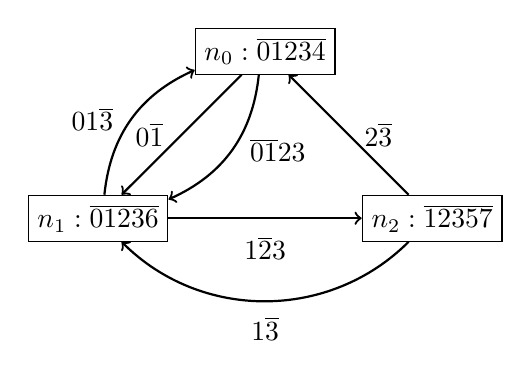
\begin{tikzpicture}[node distance = 30mm]
  \node[draw] (n0) {$n_0:\overline{01234}$};
  \node[draw,below left of=n0] (n1) {$n_1:\overline{01236}$};
  \node[draw,below right of=n0] (n2) {$n_2:\overline{12357}$};

  \draw[->,thick] (n0) -- node[left=1mm]  {$0\overline{1}$} (n1);
  \draw [->,thick] (n0) to [bend right=-30] node[right=1mm]  {$\overline{01}23$} (n1);
  \draw [->,thick] (n1) to [bend right=-30] node[left=1mm]  {$01\overline{3}$} (n0);

  \draw [->,thick] (n1) -- node[below=1mm]  {$1\overline{2}3$} (n2);
  \draw [->,thick] (n2) to [bend right=-45] node[below=2pt]  {$1\overline{3}$} (n1);

  \draw [->,thick] (n2) -- node[right=2pt]  {$2\overline{3}$} (n0);

\end{tikzpicture}
\end{minipage}

\caption{Pairing matrix} \label{fig:M1}
\end{figure}

%%% Local Variables:
%%% mode: latex
%%% TeX-master: "main"
%%% End:

%\subsection{Modeling and Symbolic Analysis of VTS: An Overview}
\label{subsec:graphmodel}

\subsection{Combinatorial problem and use of Formal methods}
\noindent The analysis of vesicle traffic systems is a difficult problem
because of the combinatorial scaling of possible traffic topologies and regulatory rules. 
%
%For example, we might want to check some conjecture of interest for all graphs of a certain structure. 
%
%If the analysis is done on a large number of graphs, the joined effect of large quantity of graphs and combinatorially many possible regulatory rules will be difficult to handle by any tool.
If the analysis is done on a large number of graphs, the joined effect of this with combinatorially many possible regulatory rules will be difficult to handle by any tool.
%
Precise analysis of the properties of the VTS would be hindered by the same reason. 

In previous work, a sampling approach was undertaken. 
%
The study used a rule-based approach~\cite{mani2016stacking}, where given an initial condition of the cell, and rules for molecular traffic, the state of each compartment in the cell is updated until a steady state is reached. 
%
With this study, statistical claims can be made, but improbable albeit biologically possible solutions could have been missed.
%
Also, there are many ways in which the dynamics of vesicle transport can be played out, while a single one was explored in this work. 
%
It is possible that a different scheme for the dynamics could lead to a different set of solutions.

%Previous analyses of vesicle traffic networks dealt with this combinatorial
%explosion by using a sampling approach~\cite{mani2016stacking}. 
%
%In these analyses, vesicle traffic is modelled as an update system. 
%
%The traffic rule specifies how the system transitions from one
%time point to the next. 
%
%Given a traffic rule and an initial condition, the system updates molecular flux of the compartments one step a time choosing one among the possibly exponential choices of the rule.
%
%The update rule defines the flux transition for the next step. 
%
%This process is performed until a steady state is reached. 
%
%
%By studying a large sample of randomly generated update rules, such analyses can make statistical claims about vesicle traffic. 
%

In contrast, here we seek understand properties of vesicle traffic networks over all possible update rules, not just for a sampled subset. 
%
We would also like to directly make statements about steady state properties, rather
than using transition dynamics to first search for steady states. 
%
Formal verification tools like model checkers, SAT and SMT solvers serve precisely this purpose. 
%
The tools model the computation symbolically for the graphs of finite size and can make prediction about the hypothesis for all possible states of the system without explicit enumeration of rules. 
%

\subsubsection{Size of the VTS system}
Let us discuss rough sizes of the system and expected behaviors.
%%
%A typical VTS may have about 10 compartments.
%%
%%Across eukaryotes, there are 20 broad SNARE varieties, though individual species can
%%contain higher numbers (humans have 41)~\cite{kloepper2007elaborate}..
%%
%The VTS may transport a large number of molecules but the molecules that
%are relevant of the control of VTS are about 50~\cite{kloepper2007elaborate}.
%%
%According to the definition the activity of molecules can be controlled by
%the presence of all other molecules.
%%
%However, in practice the activity of a molecule is controlled by
%the presence of ~2-3 other molecules.
A typical eukaryotic cell contains 9 organelles; the ER, the cis-, medial- and trans-Golgi, the early, late and recycling endosomes, the lysosome and the plasma membrane~\cite{lodish2008molecular}. 
%
The organellar content of cells vary across different organisms, for example, parasitic cells such as Trypanosomes have specialized secretory organelles called rhopteries and micronemes~\cite{gubbels2012evolution}. 
%
The organellar content may also vary across different states of the same cell, for e.g., during cell division, the Golgi apparatus disintegrates into vesicles~\cite{tang2013cell}. 
%
Also, across different cell-types, these organelles may be more or less differentiated, for example, number of stacks in the Golgi vary across different cells~\cite{polishchuk2004structural}. 
%

Going by the above description, we can assume that the VTS has of the order of 10 compartments. 
%
The VTS transports a large number of molecules but the molecules that actively control the system are in their tens [MBOC]. 
%
By definition the activity of any VTS molecules can be controlled by all other molecules.
%
However, in practice the activity of a molecule is directly controlled by 2-3 other molecules; for example, adaptor proteins are recruited to compartments by lipids of the compartment membrane and by ARF/SAR GTPases~\cite{kahn2009toward}. 
%
Some molecules, such as Rab GTPases are master regulators which control many different VTS molecules with diverse functions~\cite{zerial2001rab}. 
%
But most VTS molecules have more localized influence.
%
We use the above information during the encoding of all search problems presented later.

% i.e., formally as a boolean function that given requisite labels of nodes and vesicles that returns true if the required regulations are met. 
%
%
% Note that the formulas define among other things constraints over
% paths between nodes in the graph model of VTS. Similarly, one can
% define fusion rules as constraints over the boolean functions modeling
% the regulations.  
% For example, the steady state condition, described informally earlier, can be defined by the formula shown in Listing~1.1.
%\begin{itemize}
%\item \srivas{Detailed BIO to Graph problem}
%\end{itemize}
%Given definitions of fusion and budding rules and the steady state conditions, whether a VTS meets maximum connectivity requirement, i.e. the LGC property, can be verified by checking if the formula show in Listing~1.2 is valid.  Here we have defined the property by checking over existence of any fusion/budding rules.  We can eliminate the existential quantifier if we are interested in checking the property for a particular fusion/budding rule.
%
%\subsection{Converting the Graph Problem into Boolean SAT problem}
%\label{subsec:satproblem}
%To convert the graph problem described in sec~\ref{subsec:graphmodeling}, into a boolean SAT problem, we need to define a scheme to represent graphs and boolean functions using a suitable set of propositional variables.  In our earlier work, we modeled the graph problem in C using arrays to model graphs and boolean function.  We then used the CBMC model checker to convert the graph problem into a SAT problem.  One of the challenges we had in our earlier work is dealing with quantifiers.  Note that the connectedness property defined in Listing~1.2 has quantifier alternation.  Even if we were to eliminate the existential quantifier by instantiating the problem for a fixed set of fusion rules, we would have embedded quantifiers in the antecedent of implications.   CBMC supports only a quantifier-free logic n its assertion language.  In our earlier work we used a combination of explicit enumeration at the C-level and clever use f non-determinism to eliminate alternation of quantifiers.  This enumeration was one source of bottleneck for scaling in our earlier work.  In the current work we eliminate this bottleneck by modeling the problem directly as a SAT instance using uninterpreted functions and recursive relations.  The details of te hnew encding will described in subsequent sections.
%A VTS is {\em $k$-connected} if every pair of compartments remain reachable after dropping $k-1$ vesicles.
%
%This property of VTSs has been considered informative and studied by~\cite{shukla}.
%
%Here we have build an {\em efficient} tool that studies properties of VTSs that are not $k$-connected, from some $k$. 
\subsection{Synthesis of VTS }
\noindent The current picture of the vesicle transport network is far from complete; we do not yet know how many of the cellular proteins reach their resident compartments within the cell, and new vesicle routes are being discovered every year ~\cite{nickel2018unconventional,weill2018toolbox}. 
%
Completing the vesicle traffic network is a difficult task for the many important reasons: 
\begin{enumerate}
	\item The core vesicle transport network is conserved across eukaryotes, the traffic network in different organisms \cite{richardson2015evolutionary,nishimoto2009differential,barlow2017seeing}, and even in different cell types within an organism can be different ~\cite{stoops2014trafficking,zhou2015arp2}.
	
	\item Although the basic molecular machinery is the same for all vesicle fusion events, the details of regulation can be different~\cite{davletov2007regulation,di2010calcium}.
	
	\item Molecules can have redundant routes within the cell ~\cite{shimizu2014compensatory,nakatsukasa2014nutrient}.
	\item Behaviour of traffic molecules in vitro is different from their behaviour inside cells ~\cite{furukawa2014multiple}. 
	
	
	\item It can be difficult to distinguish between the direct and indirect effects of experiments involving knock-downs or knock outs of traffic molecules \cite{hirst2004epsinr,mishev2013small}.
\end{enumerate}

Nonetheless, completing the vesicle traffic network for different organisms is very useful. 
%
Many diseases are caused by the malfunction of the vesicle traffic network. 
%
Knowledge of the complete network would be helpful in identifying the root causes~\cite{bexiga2013human,gissen2007cargos}. 
%
At a more basic level, having complete pictures of the vesicle traffic system for various organisms and various cell-types would allow comparative studies, and therefore would allow the deduction of modes of evolution of the form of the traffic network, and would also allow us to decipher features such as parts of the traffic system that are unchanging, and therefore likely to be its core, and parts that are more plastic \cite{barlow2017seeing}.

%\subsection{Synthesis of VTS:}
%
The set of basic constraints the VTS should follow is dictated by underlying cell biology.   
%
In order to attempt to complete a given partial VTS we have to first agree on the properties that every complete VTS should follow in spite of the basic constraints. 
%
We can use our stability and k-connectivity constraints as a basis for this investigation.   
%
The incomplete VTS might not respect these constraints. 
%
In this paper, using constraints on global vesicle traffic network topology due to local molecular interactions, we take incomplete pictures of vesicle traffic networks as inputs.
%
We output various completed versions of VTS against these properties which can then be tested experimentally.
%

We have implemented the encoding in a flexible tool, which can handle a wide range of synthesis queries. 
%
We have applied our tool on several VTSs including
two found-in-nature VTSs.
%
Our experiments suggest that some of the synthesis problems are solvable by modern solvers and the synthesis technology may be useful for biological research.
%
%\begin{example}
%	%
%	In figure~\ref{fig:synth-vts}, we present a partial VTS that has 3 compartments and it's complete VTS by our tool. The synthesis is performed on the basis of steady state property and the  k-connectivity of the graph.
%	
%\end{example}
%\begin{figure}[t]
%	\centering
	%\begin{minipage}{0.45\linewidth
 \begin{subfigure}[b]{0.49\linewidth}

	\begin{tikzpicture}[->,>=stealth', auto , node distance=3.1cm,
	  thick,main node/.style={rectangle,draw}]
	 % 	\begin{scope}[]
	  \node[main node, text width=1.5cm] (pm) {PM { \^{Qa5} 
	  		                     \^{Qa7} \^{Qbc2} \^{Qbc7}}};
	  \node[main node, text width=1.5cm] (ee) [below right of=pm] {EE { \^{Qa2} \^{Qb2/3} \^{Qc2/3}}};
	  \node[main node, text width=1.5cm] (le) [above of=ee,yshift=-10mm,xshift=20mm] {LE { \^{Qa8} \^{Qb8} \^{Qc8}}};
	
	  %le <-> pm
	  \path (le) edge[bend right=55] node [above] {Qb7 Qc7} (pm);
	  %ee -> le
	  \path (ee) edge[bend right=32, text width=2.0cm] node [below,rotate=55] {\^{R8},Qa7, Qbc7,R7} (le);
	
	  %pm <-> ee
	  \path (ee) edge[bend left=32] node [below, rotate=-15] {\^{R3}} (pm);
	  \path (pm) edge[bend left=30, text width=2.0cm] node [above,rotate=-45] {\^{R2} {Qa7} Qbc7, R7, Qc7, Qa2} (ee);
	\end{tikzpicture}
  \end{subfigure}%
 % \end{scope}
%  \vspace{1.2cm}
  \begin{subfigure}[b]{0.49\linewidth}
	  \begin{tikzpicture}[->,>=stealth',auto,node distance=3.5cm,
	  thick,main node/.style={rectangle,draw}]
	 % \begin{scope}[xshift=3.5cm,yshift=0.0cm]
	  \node[main node,text width=1.5cm] (pm) {PM {\small \^{Qa5} \^{Qa7} \^{Qbc2} \^{Qbc7 ...}}};
	  \node[main node, text width=1.5cm] (ee) [below right of=pm] {EE {\small \^{Qa2} \^{Qb2/3} \^{Qc2/3} ... }};
	  \node[main node, text width=1.5cm] (le) [above of=ee,yshift=-10mm,xshift=23mm] {LE {\small \^{Qa8} \^{Qb8} \^{Qc8 ...}}};
	  
	  %le <-> pm
	  \path (le) edge[bend right=45] node [above] {Qb7 Qc7,{\color{blue} { \textbf{R7}}}} (pm);
	  
	  %le <-> ee
	  {\color{red} { \path (le) edge[bend right] node [below,rotate=50] {\color{blue} { {\textbf{\^{R8},Qa7}}}} (ee);
	  }}
	  %ee -> le
	  \path (ee) edge[bend right] node [text width=1.5cm, below,rotate=50] {\^{R8},Qa7, Qbc7,R7} (le);	  
	  
	  %pm <-> ee
	  \path (ee) edge[bend left=30] node [below, text width=2.0cm] {\^{R3, {\color{blue} { \textbf{\^{Qa2}, \^{Qa7}, \^{R2}}}}}} (pm);
	  \path (pm) edge[bend left=30] node [above,rotate=-45,text width = 2.5cm] {\^{R2} {Qa7} Qbc7, R7, Qc7, Qa2} (ee);	    
	 % \end{scope}
	 \end{tikzpicture}
  \end{subfigure}%
  \caption{An example of synthesis of edge and molecules in partial VTS.} \label{fig:synth-vts}
\end{figure}

  


The rest of the paper is organized as follows. 
%
In Sect.~\ref{sec:prelim}, we present the notations we use in this paper. 
%
In Sect.~\ref{sec:model}, we present graph model of VTSs and  properties of interest in Sect.~\ref{sec:property}.
%
%encoding of several constraints on VTSs. 
%
%In , we present the
%
In Sect.~\ref{sec:problem}, we present the complete formal problem statement of the verification properties.
%
In Sect.~\ref{sec:encoding}, we present the encoding of BMC, SMT, QBF and Synthesis into SAT, SMT and QBF satisfiability. 
%
In Sect.~\ref{sec:experiments}, we present our implementation and experimental results. 
%
In Sect.~\ref{sec:related}, we discuss related work and conclude in Sect.~\ref{sec:conclusion}.
%
%%% Local Variables:
%%% mode: latex
%%% TeX-master: "main"
%%% End:
~        
